\documentclass[12pt]{article}
\usepackage{graphicx}
\usepackage{fullpage}
\usepackage{float}
\usepackage[symbol]{footmisc}
\graphicspath{{../images/}}

\title{The Digital Age}
\author {
Kevin Yu
}

\begin{document}
\maketitle

\begin{abstract}
\end{abstract}

\section*{Introduction}

\section*{Methods}

\subsection*{Fourier Analysis: DFT, FFT}


\subsection*{Nyquist Frequency}
One of the most important concepts in digital sampling is the Nyquist criteron, which specifies the minimum frequency at which it is possible for a digitally sampled waveform to accurately reproduce the frequency composition of the actual signal. The Nyquist criteron can be put in this way: for a particular sample rate $\nu_{samp}$, only signal frequencies at or below the Nyquist rate
\begin{eqnarray}
 \nu_{nyquist} = \nu_{samp} / 2 \label{eq:nyquist}
\end{eqnarray}
can be captured by the sample. The reason for this is fairly intuitive; if one samples points separated by a time $\Delta{t}$, then any fluctuations in the signal that occur between the two samples will not be observed. To see a fluctuation in the signal, at least two points per period (one ``high" and one ``low") must be taken---this statement is equivalent to Eq.\ref{eq:nyquist}.

Failure to satisfy the Nyquist criteron will result in \textit{aliasing}, in which the sampled waveform depicts a slower frequency and possibly opposite phase to the original signal. If I ever get around to it, a artistic depiction of this phenomenon will be drawn in Figure \ref{fig:aliasing}.
\begin{figure}[H]
\center{
  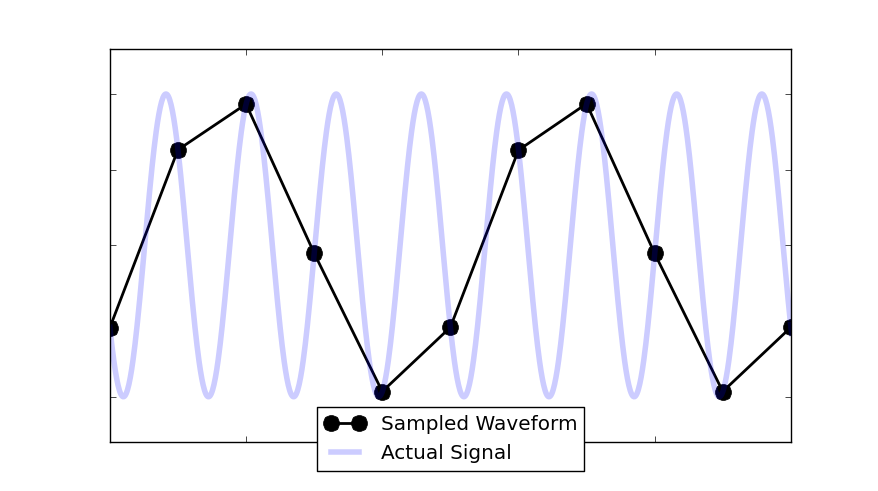
\includegraphics[width=400px]{aliasing}
}
\caption[SODUMB]{An example of aliasing. Because the sample rate is not fast enough to capture the high frequency information in the signal, the result appears to be of a slower frequency.}
\label{fig:aliasing}
\end{figure}

To demonsrate this, we use the Pulsar sampler card to take digital waveforms of incoming sine waves produced by the SRS Signal Generators. We fix our sampling rate at $\nu_{samp} = 10kHz$\footnote{This is safely below the Pulsar's maximum sampling rate of $10 MHz$}. The Nyquist frequency for this sampling rate is $\nu_{nyquist} = 5 kHz$, so will test signals at $\nu_{sig} = 1kHz$, $2kHz$, $3kHz$, $...$, $9kHz$. The sampled waveforms for these signals, as well as their power spectrum, are shown in Figure \ref{fig:nyquist}.

As can be seen from the time domain representation of the sampled waveforms, the signals from $1kHz-4kHz$ are all represented well; though the interpolated waveforms appear jagged, the underlying sinusoidal shape and frequency of the signal are clearly visible. The peaks in the power spectrum correspond well with the true frequency of its signal.

At $5 kHz$, which is exactly the Nyquist rate, the sampled waveform is a series of high and low values, with the high values always at about the same value and same for the low values. The reason they are identical is because the incoming signal is sampled at \textit{exactly} twice per period, at exactly the same point in the sinusoid's cycle each time. Because there are only two values, the shape of the waveform lacks detail---a waveform alternating between two values can be interpreted as a sine wave, a triangle wave, a square wave, etc. However, the underlying $5 kHz$ frequency is still clear in both the time domain representation and the fourier spectrum. 

Finally, the importance of the Nyquist criteron can be seen in the sampled data for $\nu_{sig} = 5 kHz$. At these signal frequencies, we no longer see spikes at the expected frequencies in the power spectrum. When we look at the sampled waveform in the time domain, the signals actually begin to look slower than the Nyquist frequency, $5 kHz$. In fact, the frequency domain representation shows that the apparent frequency turns out to be the true frequency reflected across $\nu_{nyquist}$. Additionally, the four of these sampled waveforms appear to have a $180^\circ$ phase shift relative to the signal's actual phase; this can be seen by noticing that although the actual signal begins with a downward slope, the sampled waveform begins with an upward slope.

\begin{figure}[H]
\center{
  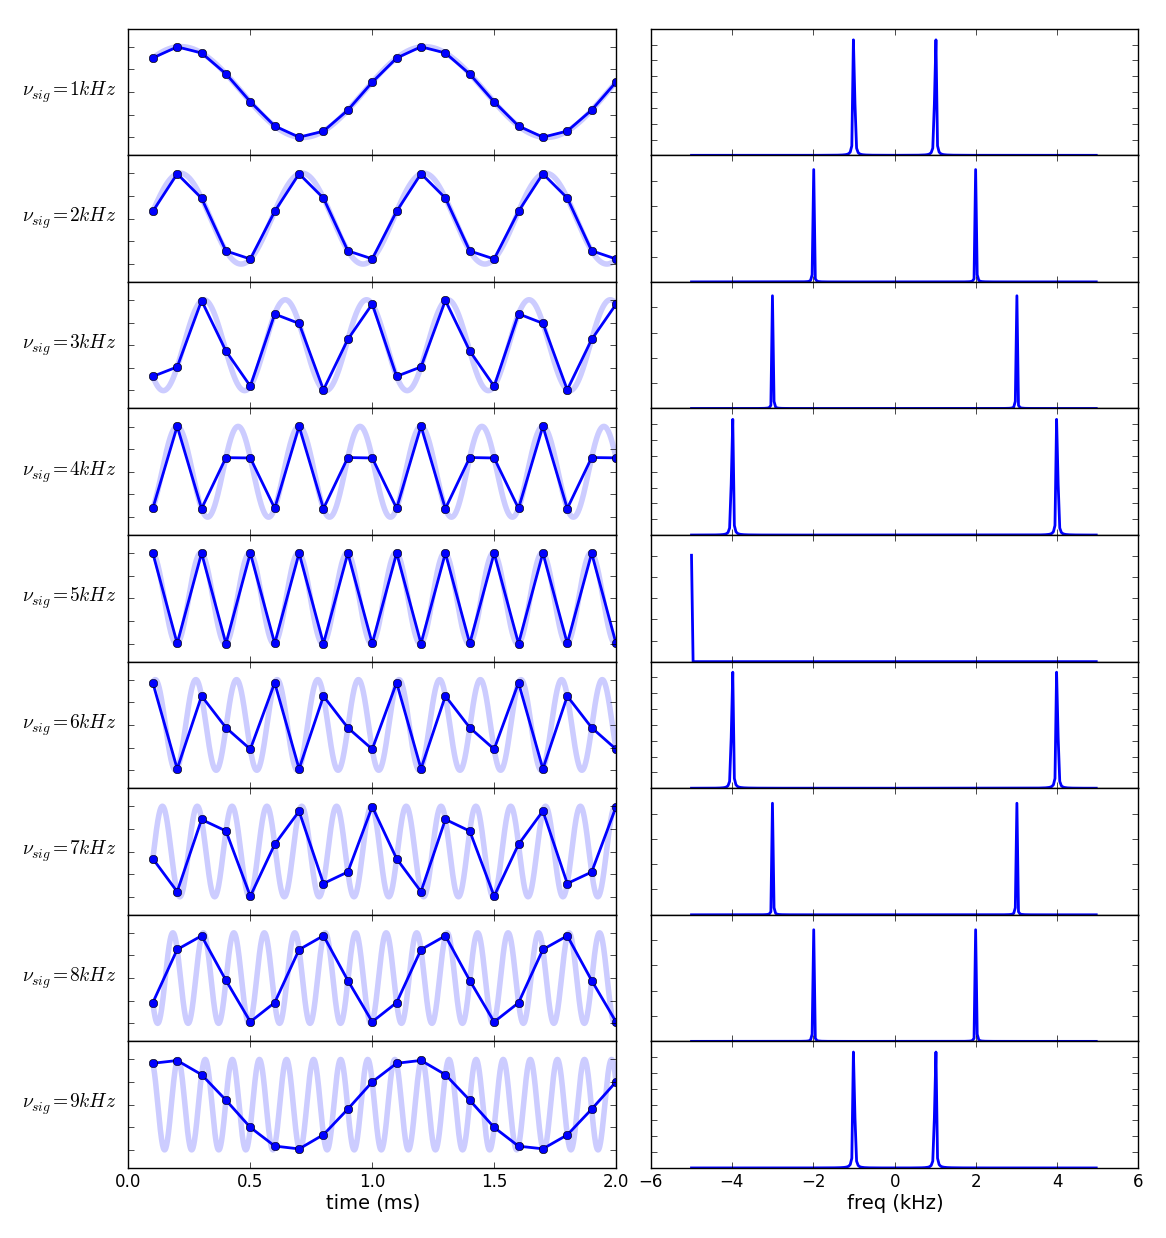
\includegraphics[width=460px]{nyquistsampling}
}
\caption[SODUMB]{Left: Time domain representation of sampled waveforms, with interpolation, for signal frequencies from $1 kHz$ to $9 kHz$, sampled at a rate $\nu_{samp}=10 MHz$. Aliasing can be seen for signal frequencies greater than $\nu_{nyquist}=5 MHz$. A representation of the actual signal is overlayed in a lighter shade. Right: The corresponding power spectrum for sampled waveforms on the left. For signal frequencies greater than the Nyquist rate, the observed frequencies are the actual frequencies reflected over $\nu_{nyquist}$. The power spectrum for $\nu_{sig}=5MHz$ is missing a spike at $5MHz$ due to the nature of the \texttt{fft} program used, which is asymmetric around zero in that it omits the final frequency point on the positive side.}
\label{fig:nyquist}
\end{figure}

\subsection*{Mixing} 

A local oscillator, or LO, is a signal used to convert an incoming signal to a different frequency. When we \textit{mix} two signals, $f$ and $g$, we multiply them in the time domain, which is equivalent to convolving them in the frequency domain.

In this lab, we begin by using an analog mixer---the ZAD-1. As per the lab manual instructions, we will pick a $\nu_{LO}$ and mix it with another signal at chosen frequencies. The first time, we will mix it with a signal of frequency $\nu_{sig} = \nu_{LO} + \delta \nu$, and the second time we will mix it with a signal of frequency $\nu_{sig} = \nu_{LO} - \delta \nu$. Because the two signals, our signal and our local oscillator, will be set by the SRS Signal Generators, they will both be real and thus consist of both $e^{i\omega t}$ and $e^{-i\omega t}$ components. Thus, after mixing the output should be composed of four frequencies, $-\nu_{LO} - \nu_{sig}$, $-\nu_{LO} + \nu_{sig}$, $\nu_{LO} - \nu_{sig}$, and $\nu_{LO} + \nu_{sig}$.

Looking at the positive $\nu_{LO}$ frequencies, we see that the output will be split into a lower sideband---$\nu_{LO} - \nu_{sig}$---and an upper sideband---$\nu_{LO} + \nu_{sig}$. This is a double sideband (DSB) mixer. A single sideband (SSB) mixer would require mixing with pure sinusoids of the form $e^{i\omega t}$, which have both a real and imaginary part, and would remove half of the sidebands created.

We use ... and collect $N=16384$ data points, sampling for N times delta t seconds. 
WHAT VALUES DID WE USE?
WHAT DID WE SEE?

\begin{figure}[H]
\center{
  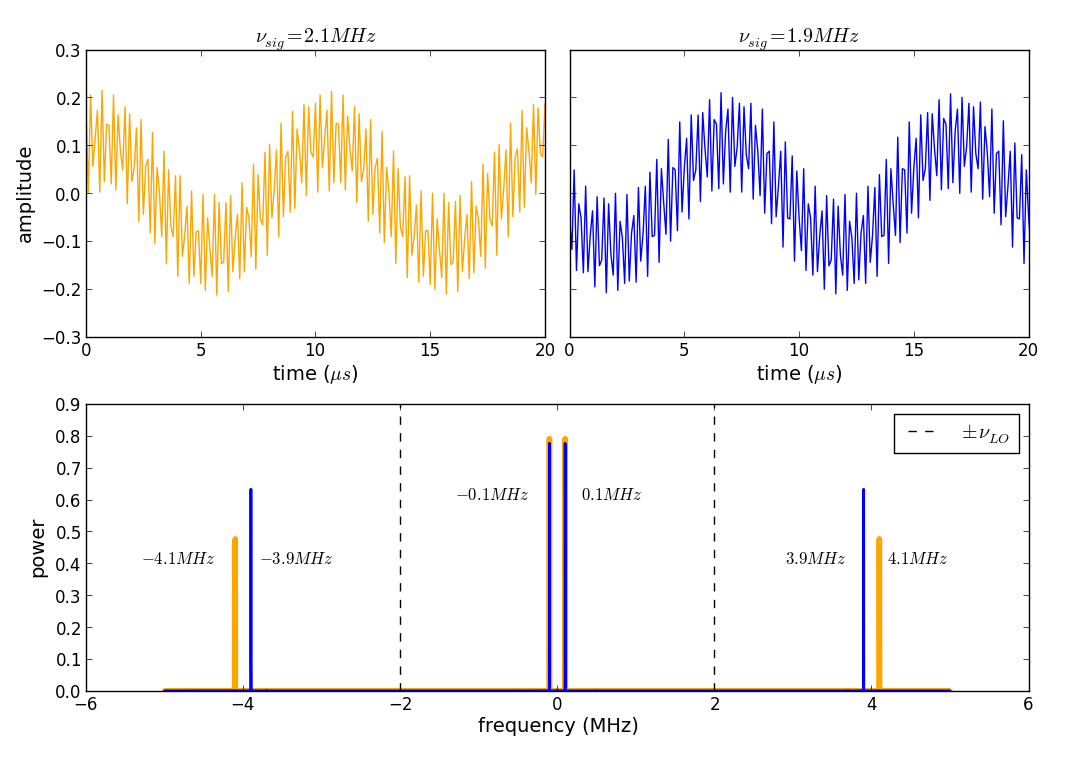
\includegraphics[width=460px]{analogmixing}
}
\caption[SODUMB]{Top Left: Output from analog mixer with $\nu_{sig}=2.1MHz$ and $\nu_{LO}=2MHz$, digitally sampled at $10 MHz$. Top Right: Output from analog mixer for with $\nu_{sig}=1.9MHz$ and $\nu_{LO}=2MHz$. Bottom: The power spectrum for both of the outputs. Notice that both results have spectral features at $\pm 0.1 MHz$ due to the fact that the mixers produce frequencies at $\nu_{LO} \pm \nu_{sig}$ as well as $-\nu_{LO} \pm \nu_{sig}$}
\label{fig:analogmixing}
\end{figure}


\subsection*{Digital Mixing Using the ROACH}
The ROACH, is a system consisting of a CPU running a Linux kernel and an FPGA, which can be configured to perform tasks with many logic gates running in parallel, synchronized in this lab by a $200 MHz$ clock. We can connect with it remotely and configure our data collection by writing to the FPGA's registers. The ADC output is written into block random access memory (BRAM), which once full can be copied out of the ROACH for analysis. 

\subsubsection*{Double Sideband (DSB)}
In the last section, we used an analog mixer to mix our signals with frequency $\nu_{LO}$ and $\nu_{sig}$. The ROACH is capable of digitally mixing the two signals when the inputs are connected to ports 2 and 3. Using the same frequencies for our signal and local oscillator, we expect to see a similar result to the analog mixer. ADD FREQUENCIES AND OTHER QUALTITAVEI EXPECTATIONS. We will use a clock rate of $200 MHz$ with the ROACH for sampling.

\begin{figure}[H]
\center{
  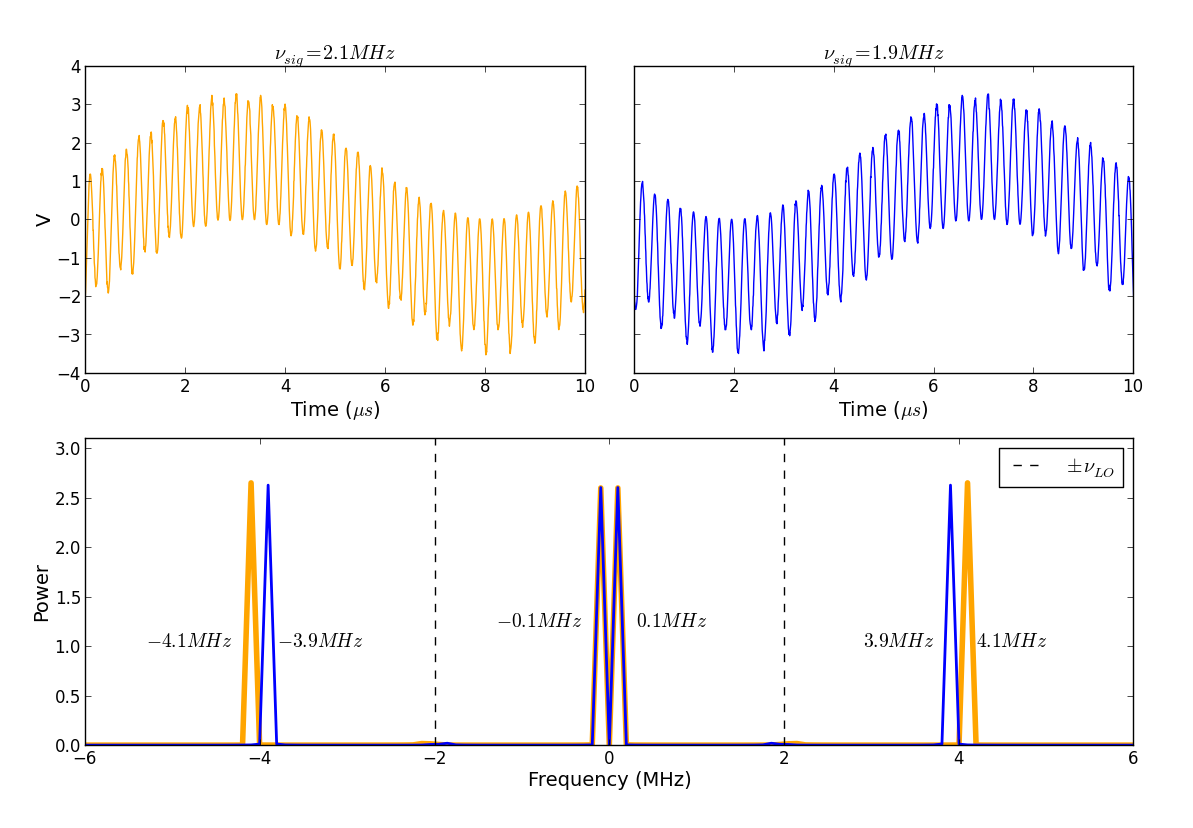
\includegraphics[width=460px]{digitalmixing}
}
\caption[SODUMB]{Similar to Figure \ref{fig:analogmixing}, this time mixing digitally using the ROACH. Top Left: Output of digital mixer with $\nu_{sig}=2.1MHz$ and $\nu_{LO}=2MHz$, sampled at $200 MHz$. Top Right: Output from analog mixer for with $\nu_{sig}=1.9MHz$ and $\nu_{LO}=2MHz$. Bottom: The power spectrum for both of the outputs. The spectral features occur at the same frequencies as in the analog case of Figure \ref{fig:analogmixing}. The peaks in the spectrum consist of a single datapoint each---the reason they look wider than in Figure \ref{fig:analogmixing} is that the limited size of the ROACH's BRAM only allowed us to sample for about one period which limited our resolution in the frequency domain.}
\label{fig:digitalmixing}
\end{figure}

The results of digital mixing with these signal frequencies can be seen in Figure \ref{fig:digitalmixing}. The waveform and power spectrum are very similar to the results of the analog mixing case in Figure \ref{fig:analogmixing}. However, there are a couple differences that can be seen in the power spectrum by noticing that the peaks seem wider than their counterparts in the analog mixing case.

The reason for these apparently wider peaks is a lower frequency resolution due to a limited sample size. When data collection is triggered on the ROACH, data points are collected and stored in BRAM until the BRAM is full, limiting the number of data points that we can take. Apparently, the BRAM can only store 2048 32-bit signed integers, meaning if we take samples at $200 MHz$ we can sample for $10.24$ $\mu s$. In comparison, when we sampled the output of our analog mixer using the Pulsar card, we took 16384 values at $10 MHz$, meaning we sampled for $1$ $ms$, one hunderd times longer. Because of this, our resolution in the frequency domain for digitally sampling on the ROACH is one hundred times lower than in the earlier section, which is why the peaks in the spectrum look so fat.

One way to solve this would be to decrease the clock rate much lower than $200 MHz$, so that the BRAM does not fill up as quickly. This would allow us to take data for a longer period of time.

. We use .... . The plots ... . The analysis ... .

\subsubsection*{Single Sideband (SSB)}
In the DSB, we mixed our signal $f$ with a wave of the form $\cos(\omega t)$. Because the $\cos$ has no imaginary part, we essentially mix our signal with both $e^{i \omega t}$ and $e^{-i \omega t}$ waves, creating the upper and lower sidebands, respectively. Using the ROACH, we will be able to mix with both a $\cos$ and $\sin$ wave simultaneously. Combining the resulting waveforms using the relationship TODO: move this to a theory paragraph before this)
\begin{eqnarray}
f(t) e^{i\omega t} = [f(t) \cos(\omega t)] + i [f(t) \sin(\omega t)] \label{eq:mixingexp}
\end{eqnarray}
The ROACH does not output the complex result of the mixing; instead, it mixes the signal simultaneously with samples from a sine and a cosine local oscillator (two sinusoids a quarter period out of phase). These two outputs are stored in separates BRAMs. With those sampled datapoints, we can then programmatically combine them using Eq.\ref{eq:mixingexp} to see the full, complex result.

The frequency of the LO is set by the ROACH's sampling clock and the value written to the \textit{lo\_freq} register, which I will call $x$. To do this, the interval of $0$ to $2\pi$ is divided into 256 steps; i.e. $0, \frac{2\pi}{256}, \frac{2\pi}{128}, \frac{2\pi}{64}$, etc. 

Each clock cycle, the ROACH increments its current position in the interval by $x$ steps. The FPGA then evaluates $\cos$ and $\sin$ at that value to be mixed with the next sampled point of the incoming signal. Thus, the entire period of $2\pi$ is completed in $256/x$ steps. With a clock rate of $\nu_{samp}$, the frequency of the LO generated in this fashion is
\begin{eqnarray}
\nu_{LO} = \frac{x}{256} * \nu_{samp}
\end{eqnarray}
To demonstrate this digital SSB mixer, we generate a $6MHz$, $0$ dbm signal with the SRS and mix it with the LO frequencies listed below, for a $200 MHz$ clock rate. Because the signal generated by the SRS will contain both ``positive" and ``negative" frequencies, as it is simply a cosine signal, we expect to see two frequencies in the output after combining the real and imaginary parts: $\pm \nu_{sig} + \nu_{LO}$. As you can see in the table, none of these expected frequencies come close to our Nyquist rate of $100 MHz$.
\begin{center}
  \begin{tabular}{ c | c | c }
    $x$ & $\nu_{LO}$ [$MHz$] & $\nu_{output} = \nu_{LO} \pm \nu{sig}$ [$MHz$]\\ \hline
    $1$ & $0.782 $ & $6.782$, $-5.218 $ \\
    $2$ & $1.563 $ & $7.563$, $-4.437$\\
    $4$ & $3.125 $ & $9.125$, $-2.875$ \\
    $16$ & $12.5 $ & $18.5$, $-6.5$\\
  \end{tabular}
\end{center}

Figure \ref{fig:ssb} illustrates the result of digitally mixing for the third case, $\nu_{LO} = 3.125 MHz$. 

\begin{figure}[H]
\center{
  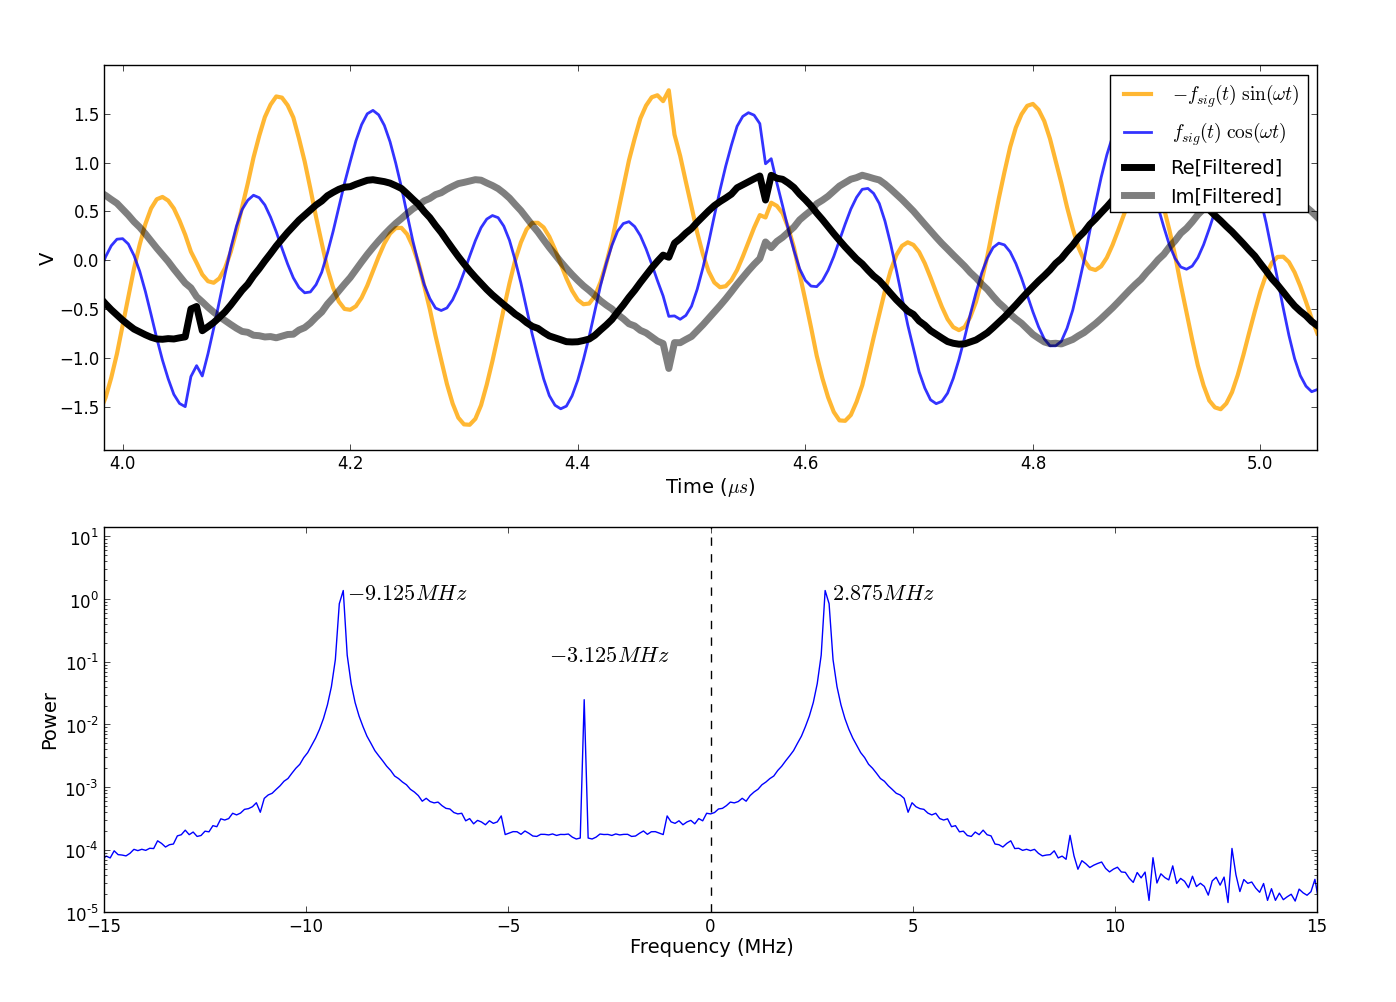
\includegraphics[width=460px]{ssb}
}
\caption[SODUMB]{Top: The result of digitally mixing a $6 MHz$ signal with a $3.125 MHz$ local oscillator on the ROACH. The blue line represents the real part, Re${[f(t)e^{i\omega t}]} = f(t) \cos(\omega t)$, and the orange line represents the imaginary part, Im${[f(t)e^{i\omega t}]} = f(t) \sin(\omega t)$. Bottom: Power spectrum of the complex result above. There are clear peaks at $\nu_{LO} \pm \nu_{sig}$, as well as a small peak at $\nu_{LO}$ from the LO signal slipping through.}
\label{fig:ssb}
\end{figure}

DISCUSS RESULTS OF
COMPLEXLY MIXED SAMPLE
- APPLY FOURIER FILTER TO IT
DISCUSS ADVANTAGE AND DISADVANTAGE OF DSB AND SSB

\subsection*{FIR Filter}
We can implement an FIR, or Finite Impulse Response, filter using the FPGA. The FIR filter allows us to convolve an incoming signal with a custom waveform in the time domain \textit{as the signal is sampled}. Our FIR filter will have 8 taps; meaning we choose 8 real and 8 imaginary coefficients to represent the filter. As the signal is sampled, the FPGA multiplies each of the last 8 points taken with their corresponding coefficients, and sums them up. Each clock cycle, a new point is sampled and the process is repeated and another sum is taken. The net effect is that we are essentially dragging, or \textit{convolving}, the incoming signal across our filter. The sums are largest at times when the signal ``looks like" our filter, and smallest when the sample does not resemble our filter---thus, the FIR filter picks out portions of the signal most similar to the filter shape.

\subsubsection*{Choosing Coefficients}
We use this functionality to implement a bandpass filter. To choose coefficients for the FIR filter, we first create our bandpass in the frequency domain---a square spectrum centered around a certain frequency---and apply the inverse fourier transform to it to get the filter in the time domain. Since we are working digitally, we will only choose 8 points (Figure TODO) of the filter so that when we do the inverse discrete fourier transform we wind up with coefficients, with both real and imaginary components, at the 8 time steps (LOOKUP CORRECT TERMINOLOGY).

Our bandpass in this experiment is a 5/8-band filter, centered around $0 Hz$. Since our clock/sample rate is $200MHz$, the Nyquist rate is $100MHz$ and the frequency range that we will concern ourselves with is the range $-100MHz$ to $100 MHz$. The 5/8-band filter will be a filter with a full response in 5/8 of that range centered around 0, or from $-62.5MHz$ to $62.5 MHz$. Elsewhere, the filter's response should be zero, as depicted in Figure TODO. To be able to take the discrete inverse fourier transform of this, we need to take 8 equally spaced samples from this ideal response. Using NumPy's fft module, we need to choose the points at frequencies listed in Table X to produce a time domain waveform with points separated by $\frac{1}{200MHz} = 5 ns$.

\begin{center}
  \begin{tabular}{ c | c }
    $\nu$ [MHz] & Power \\ \hline
    $-100$ & $0 $\\
    $-75$ & $0 $\\
    $-50$ & $1 $\\
    $-25$ & $1 $ \\
    $0$ & $1 $\\
    $25$ & $1 $  \\
    $50$ & $1$ \\
    $75$ & $0 $ \\
  \end{tabular}
  $\rightarrow$ [Inverse DFT] $\rightarrow$
  \begin{tabular}{c | l | c }
    t (ns)& Real Coeff. & Imag. Coeff.\\ \hline
    0 & \texttt{0.125} & $0$ \\
    5 & \texttt{-0.0517...}  & $0$ \\
    10 & \texttt{-0.125} & $0$ \\
    15 & \texttt{0.3017...} & $0$ \\
    20 & \texttt{0.625} & $0$ \\
    25 & \texttt{0.3017...} & $0$ \\
    30 & \texttt{-0.125} & $0$ \\
    35 & \texttt{-0.0517...} & $0$ \\
  \end{tabular}
\end{center}
\footnote{uh. precision was left down to the lowest bit. see appendix for how to convert these to 18 bit signed fixed point}

One thing to note is that the imaginary coefficients are all zero. This can be understood by noticing that the frequency spectrum that we created is symmetric around zero, meaning the spikes at positive frequencies have corresponding spikes at their negative frequency. As we have seen earlier in the lab in our SSB and DSB mixers, this symmetry between positive and negative frequency can be created with an entirely real wave (sine component zero). Explain this better later.

The discrete points chosen for the power spectrum are plotted in Figure TODO on top of the ideal 5/8-band filter. Similarly, Figure TODO shows the coefficients we used for the time domain filter on top of the ideal time domain waveform of a 5/8-band filter. As you can see, we do not have a lot of freedom with the points we choose so it will not be perfect.
 
PLOT DESIRED BANDPASS VS ACTUAL BANDPASS

\subsection*{Testing Filter Response}
To test our FIR filter's response as a function of frequency, we want to compare how the power spectrum of a waveform looks with and without the filter applied. For purposes of this experiment, I will define the response of the waveform at a frequency $\nu$ to be the magnitude of a spike at $\nu$ in the power spectrum \textit{with the filter}, divided by the magnitude of the spike at $\nu$ \textit{without the filter}. For example, If the waveform has a large spike at a frequency $10 MHz$ without the filter, but a spike half as large at $10 MHz$ with the filter, then the respnose of the filter at $10 MHz$ is $0.5$. 

The way we can see the expected magnitude in the power spectrum is by using the FIR filter with all coefficients set to zero except for one, set to the maximal possible value (close to one). This essentially reproduces the original signal as output because the FIR is simply convoluting the incoming signal with a delta function of magnitude 1---each point is simply recreated in the output.

To probe many frequencies in our range of $-100 MHz$ to $100 MHz$, we will use the digital SSB mixing techniques of the previous section. We will use a $25 MHz$ signal at $0$ dBm, mixed with LO frequencies ranging from $5 MHz$ to $X MHz$. Since we will combine real and imaginary parts programmatically, we can add them in this form
\begin{eqnarray}
f(t) e^{i\omega t} = [f(t) \cos(\omega t)] + i [f(t) \sin(\omega t)] \label{eq:mixingexp}
\end{eqnarray}
to produce upper sideband frequencies relative to the signal, or subtract them like this
\begin{eqnarray}
f(t) e^{-i\omega t} = [f(t) \cos(\omega t)] - i [f(t) \sin(\omega t)] \label{eq:mixingexp}
\end{eqnarray}
to produce lower sideband frequencies. The exact LO frequencies, and the corresponding expected output frequencies, are enumerated in the upcoming table. For each LO frequency, will collect data twice, once with the coefficients in table X for our 5/8-band filter, and again with all coefficients zero except for one (to normalize the output strength). An example of this comparison is in Figure TODO.


TESTING THE RESPONSE (HOW TO NORMALIZE)

\section*{Results}

\section*{Conclusion}

\section*{Appendix}
\subsection*{Converting FIR Coefficients to Binary}
The FIR reads 18 bit\footnote{The register holds 32 bits but only 18 bits are used.}, fixed point, 2's complement numbers from the \texttt{coeff} registers, with 17 digits after the binary point. The smallest bit, therefore, will represent the value $2^{-17}$, and the range of values that can be represented go from $-1$ to $1-2^{-17}$. A easy way to convert a decimal value into this odd representation is to divide that number by $2^{-17}$, and then fill in the preceding bits with zeroes up to the full 32 bits.

This table shows the coefficients\footnote{I truncated the decimal for sake of space. However, the coefficients were determined using \texttt{np.fft} with floating point precision; the binary and hex columns include as much precision as NumPy was willing to offer.} we wanted to use in our 5/8-band filter, as well as their binary representation in this representation and their hexadecimal representation.

\begin{center}
  \begin{tabular}{ l | c | c }
    Coeff. & Binary & Hex\\ \hline
    \texttt{-0.0517...}  &  \texttt{1.11110010101111101} & \texttt{0x3e57d}\\
    \texttt{-0.125} &  \texttt{1.11100000000000000} & \texttt{0x3c000}\\
    \texttt{0.125} & \texttt{0.00100000000000000} & \texttt{0x04000}\\
    \texttt{0.3017...} &  \texttt{0.01001101010000010} & \texttt{0x09a82}\\
    \texttt{0.625} &  \texttt{0.10100000000000000} & \texttt{0x14000}\\
   \end{tabular}
\end{center}

\section*{Acknowledgement}
I would like to thank my lab partners Maissa and Sal for their work in getting us through this lab. Also thanks to the lab instructors Aaron Parsons, Karto Keating, and Baylee Bordwell for teaching us the lab material, helping us with debugging the ROACH, and sustaining us with baked goods. Especially to Karto for providing us with with the now defunct \texttt{set\_srs}, which automagically just worked and made automating data collection so much easier!
All figures were done in Python using the Numpy and Matplotlib libraries.

\end{document}